%!TEX root = ../fro.tex
\chapter{Programmazione Lineare Intera}

\Es
\begin{gather*}
x_{2} \leq \frac{1}{5} x_{1} +4\\
x_{2} \leq -2x_{1} +\frac{19}{2}\\
x_{2} \geq x_{1} -1
\end{gather*}

\begin{figure}[htpb]
	\centering
	\tikzset{every picture/.style={line width=0.75pt}} %set default line width to 0.75pt        

	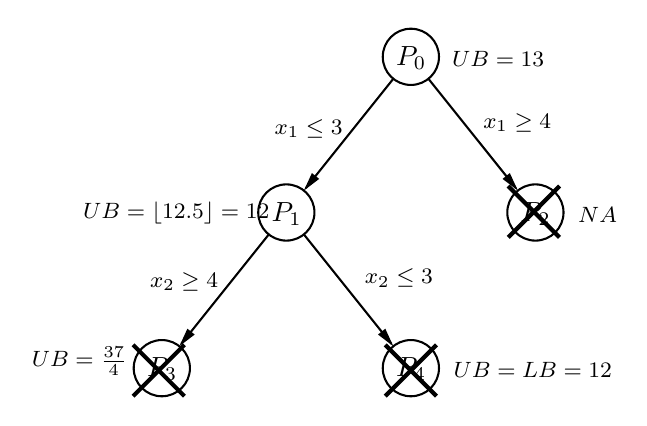
\begin{tikzpicture}[x=0.75pt,y=0.75pt,yscale=-0.75,xscale=0.75]
	%uncomment if require: \path (0,340); %set diagram left start at 0, and has height of 340

	%Straight Lines [id:da8256496838848162] 
	\draw [line width=1.5]    (355,146) -- (388,179) ;
	%Straight Lines [id:da14854697063972377] 
	\draw [line width=1.5]    (388,146) -- (355,179) ;
	%Straight Lines [id:da038487184733093205] 
	\draw [line width=1.5]    (276,248) -- (309,281) ;
	%Straight Lines [id:da09421605800632826] 
	\draw [line width=1.5]    (309,248) -- (276,281) ;
	%Straight Lines [id:da7070304946661545] 
	\draw [line width=1.5]    (114,248) -- (147,281) ;
	%Straight Lines [id:da48001648506360284] 
	\draw [line width=1.5]    (147,248) -- (114,281) ;

	% Text Node
	\draw    (292.5, 63) circle [x radius= 18.06, y radius= 18.06]   ;
	\draw (281,54.4) node [anchor=north west][inner sep=0.75pt]    {$P_{0}$};
	% Text Node
	\draw    (212.5, 163) circle [x radius= 18.06, y radius= 18.06]   ;
	\draw (201,154.4) node [anchor=north west][inner sep=0.75pt]    {$P_{1}$};
	% Text Node
	\draw    (372.5, 163) circle [x radius= 18.06, y radius= 18.06]   ;
	\draw (361,154.4) node [anchor=north west][inner sep=0.75pt]    {$P_{2}$};
	% Text Node
	\draw    (132.5, 263) circle [x radius= 18.06, y radius= 18.06]   ;
	\draw (121,254.4) node [anchor=north west][inner sep=0.75pt]    {$P_{3}$};
	% Text Node
	\draw    (292.5, 263) circle [x radius= 18.06, y radius= 18.06]   ;
	\draw (281,254.4) node [anchor=north west][inner sep=0.75pt]    {$P_{4}$};
	% Text Node
	\draw (317,57.4) node [anchor=north west][inner sep=0.75pt]  [font=\footnotesize]  {$UB=13$};
	% Text Node
	\draw (80,154.4) node [anchor=north west][inner sep=0.75pt]  [font=\footnotesize]  {$UB=\lfloor 12.5\rfloor =12$};
	% Text Node
	\draw (398,157.4) node [anchor=north west][inner sep=0.75pt]  [font=\footnotesize]  {$NA$};
	% Text Node
	\draw (318,257.4) node [anchor=north west][inner sep=0.75pt]  [font=\footnotesize]  {$UB=LB=12$};
	% Text Node
	\draw (47,247.4) node [anchor=north west][inner sep=0.75pt]  [font=\footnotesize]  {$UB=\frac{37}{4}$};
	% Text Node
	\draw (337,97.4) node [anchor=north west][inner sep=0.75pt]  [font=\footnotesize]  {$x_{1} \geq 4$};
	% Text Node
	\draw (203,101.4) node [anchor=north west][inner sep=0.75pt]  [font=\footnotesize]  {$x_{1} \leq 3$};
	% Text Node
	\draw (261,197.4) node [anchor=north west][inner sep=0.75pt]  [font=\footnotesize]  {$x_{2} \leq 3$};
	% Text Node
	\draw (123,199.4) node [anchor=north west][inner sep=0.75pt]  [font=\footnotesize]  {$x_{2} \geq 4$};
	% Connection
	\draw    (281.22,77.1) -- (225.03,147.33) ;
	\draw [shift={(223.78,148.9)}, rotate = 308.66] [fill={rgb, 255:red, 0; green, 0; blue, 0 }  ][line width=0.08]  [draw opacity=0] (12,-3) -- (0,0) -- (12,3) -- cycle    ;
	% Connection
	\draw    (303.78,77.1) -- (359.97,147.33) ;
	\draw [shift={(361.22,148.9)}, rotate = 231.34] [fill={rgb, 255:red, 0; green, 0; blue, 0 }  ][line width=0.08]  [draw opacity=0] (12,-3) -- (0,0) -- (12,3) -- cycle    ;
	% Connection
	\draw    (201.22,177.1) -- (145.03,247.33) ;
	\draw [shift={(143.78,248.9)}, rotate = 308.66] [fill={rgb, 255:red, 0; green, 0; blue, 0 }  ][line width=0.08]  [draw opacity=0] (12,-3) -- (0,0) -- (12,3) -- cycle    ;
	% Connection
	\draw    (223.78,177.1) -- (279.97,247.33) ;
	\draw [shift={(281.22,248.9)}, rotate = 231.34] [fill={rgb, 255:red, 0; green, 0; blue, 0 }  ][line width=0.08]  [draw opacity=0] (12,-3) -- (0,0) -- (12,3) -- cycle    ;

	\end{tikzpicture}
\end{figure}
\FloatBarrier

Ottimo: $12,( 3,3)$.

\begin{figure}
\centering
\begin{subfigure}{.5\textwidth}
  \centering
  \includegraphics[width=\linewidth]{1-1}
\end{subfigure}%
\begin{subfigure}{.5\textwidth}
  \centering
  \includegraphics[width=\linewidth]{1-2}
\end{subfigure}
\end{figure}
\FloatBarrier

\Es

\begin{figure}[htpb]
	\centering
	\tikzset{every picture/.style={line width=0.75pt}} %set default line width to 0.75pt        

	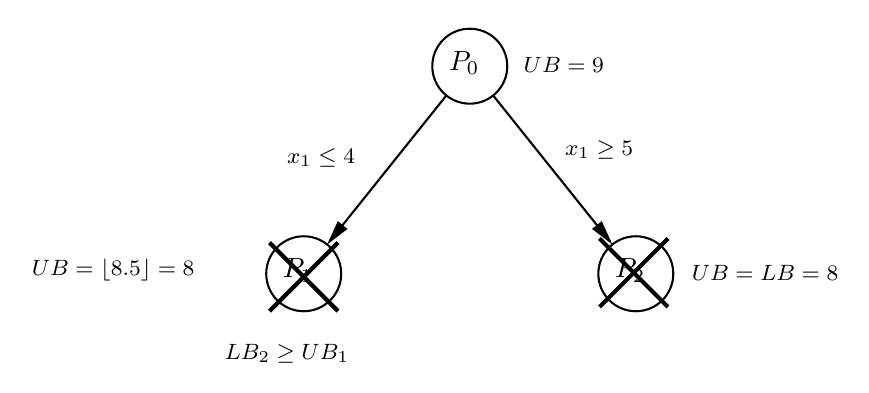
\begin{tikzpicture}[x=0.75pt,y=0.75pt,yscale=-1,xscale=1]
	%uncomment if require: \path (0,255); %set diagram left start at 0, and has height of 255

	%Straight Lines [id:da31633087052970965] 
	\draw [line width=1.5]    (355,146) -- (388,179) ;
	%Straight Lines [id:da4125010004484957] 
	\draw [line width=1.5]    (388,146) -- (355,179) ;
	%Straight Lines [id:da7570488418846992] 
	\draw [line width=1.5]    (196,148) -- (229,181) ;
	%Straight Lines [id:da8927568555222583] 
	\draw [line width=1.5]    (229,148) -- (196,181) ;

	% Text Node
	\draw    (292.5, 63) circle [x radius= 18.06, y radius= 18.06]   ;
	\draw (281,54.4) node [anchor=north west][inner sep=0.75pt]    {$P_{0}$};
	% Text Node
	\draw    (212.5, 163) circle [x radius= 18.06, y radius= 18.06]   ;
	\draw (201,154.4) node [anchor=north west][inner sep=0.75pt]    {$P_{1}$};
	% Text Node
	\draw    (372.5, 163) circle [x radius= 18.06, y radius= 18.06]   ;
	\draw (361,154.4) node [anchor=north west][inner sep=0.75pt]    {$P_{2}$};
	% Text Node
	\draw (317,57.4) node [anchor=north west][inner sep=0.75pt]  [font=\footnotesize]  {$UB=9$};
	% Text Node
	\draw (80,154.4) node [anchor=north west][inner sep=0.75pt]  [font=\footnotesize]  {$UB=\lfloor 8.5\rfloor =8$};
	% Text Node
	\draw (398,157.4) node [anchor=north west][inner sep=0.75pt]  [font=\footnotesize]  {$UB=LB=8$};
	% Text Node
	\draw (337,97.4) node [anchor=north west][inner sep=0.75pt]  [font=\footnotesize]  {$x_{1} \geq 5$};
	% Text Node
	\draw (203,101.4) node [anchor=north west][inner sep=0.75pt]  [font=\footnotesize]  {$x_{1} \leq 4$};
	% Text Node
	\draw (173,195.4) node [anchor=north west][inner sep=0.75pt]  [font=\footnotesize]  {$LB_{2} \geq UB_{1}$};
	% Connection
	\draw    (281.22,77.1) -- (225.03,147.33) ;
	\draw [shift={(223.78,148.9)}, rotate = 308.66] [fill={rgb, 255:red, 0; green, 0; blue, 0 }  ][line width=0.08]  [draw opacity=0] (12,-3) -- (0,0) -- (12,3) -- cycle    ;
	% Connection
	\draw    (303.78,77.1) -- (359.97,147.33) ;
	\draw [shift={(361.22,148.9)}, rotate = 231.34] [fill={rgb, 255:red, 0; green, 0; blue, 0 }  ][line width=0.08]  [draw opacity=0] (12,-3) -- (0,0) -- (12,3) -- cycle    ;

	\end{tikzpicture}
\end{figure}
\FloatBarrier

Ottimo: $8,( 5,-1)$.

\fg{0.5}{2}

\Es

Rilassamento continuo:
\begin{equation*}
x_{1} =0\ \ x_{2} =\frac{7}{2} \ \ s_{1} =0\ \ s_{2} =\frac{3}{2}
\end{equation*}
Equazioni dei tagli:
\begin{equation*}
\begin{array}{ l l l l l c }
x_{2} +x_{1} +\frac{1}{2} s_{1} =\frac{7}{2} & \rightarrow  & x_{2} +x_{1} +\left\lfloor \frac{1}{2}\right\rfloor s_{1} \leq \left\lfloor \frac{7}{2}\right\rfloor  & \rightarrow  & x_{2} +x_{1} \leq 3 & \boxed{x_{1} +x_{2} \leq 3}\\
s_{2} -x_{1} +\frac{1}{2} s_{1} =\frac{3}{2} & \rightarrow  & s_{2} -x_{1} +\left\lfloor \frac{1}{2}\right\rfloor s_{1} \leq \left\lfloor \frac{3}{2}\right\rfloor  & \rightarrow  & s_{2} -x_{1} \leq 1 & \\
 &  &  &  & s_{2} =2x_{1} +x_{2} -2 & 
\end{array}
\end{equation*}
Ottimo: $-6,( 0,3)$.

\fg{0.3}{3}

\Es

Rilassamento continuo:
\begin{equation*}
x_{1} =0\ \ x_{2} =\frac{9}{2} \ \ s_{1} =0\ \ s_{2} =\frac{5}{2}
\end{equation*}
Equazioni dei tagli:
\begin{equation*}
\begin{array}{ l l l l l c }
x_{2} +\frac{1}{2} s_{1} =\frac{9}{2} & \rightarrow  & x_{2} +\left\lfloor \frac{1}{2}\right\rfloor s_{1} \leq \left\lfloor \frac{9}{2}\right\rfloor  & \rightarrow  & x_{2} \leq 4 & \boxed{x_{2} \leq 4}\\
s_{2} +2x_{1} -\frac{1}{2} s_{1} =\frac{5}{2} & \rightarrow  & s_{2} +2x_{1} -\left\lfloor \frac{1}{2}\right\rfloor s_{1} \leq \left\lfloor \frac{5}{2}\right\rfloor  & \rightarrow  & s_{2} +2x_{1} -s_{1} \leq 2 & 
\end{array}
\end{equation*}
Ottimo: $-8,( 0,4)$.

\fg{0.6}{4}

\Es

$B=13$.
\begin{equation*}
\arraycolsep=2pt\def\arraystretch{1.6}
\begin{array}{ c|c c c c }
p_{i} & 16 & 9 & 12 & 2\\
\hline
w_{i} & 8 & 6 & 7 & 2\\
\hline
\frac{p_{i}}{w_{i}} & 2 & \frac{3}{2} & \frac{12}{7} & 1\\
\hline
 & x_{1} & x_{2} & x_{3} & x_{4}
\end{array}
\end{equation*}
Ordino
\begin{equation*}
x_{1} ,x_{3} ,x_{2} ,x_{4}
\end{equation*}

\begin{figure}[htpb]
	\centering
	\tikzset{every picture/.style={line width=0.75pt}} %set default line width to 0.75pt        

	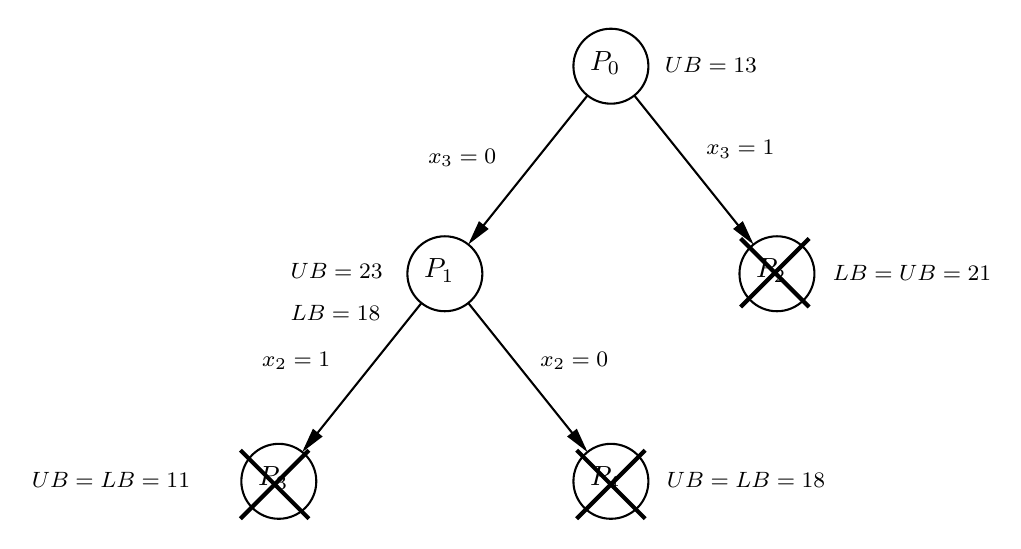
\begin{tikzpicture}[x=0.75pt,y=0.75pt,yscale=-1,xscale=1]
	%uncomment if require: \path (0,340); %set diagram left start at 0, and has height of 340

	%Straight Lines [id:da902458193250876] 
	\draw [line width=1.5]    (355,146) -- (388,179) ;
	%Straight Lines [id:da770061225974817] 
	\draw [line width=1.5]    (388,146) -- (355,179) ;
	%Straight Lines [id:da6732168860960122] 
	\draw [line width=1.5]    (276,248) -- (309,281) ;
	%Straight Lines [id:da5913463822053582] 
	\draw [line width=1.5]    (309,248) -- (276,281) ;
	%Straight Lines [id:da8203822268133403] 
	\draw [line width=1.5]    (114,248) -- (147,281) ;
	%Straight Lines [id:da5206633509023615] 
	\draw [line width=1.5]    (147,248) -- (114,281) ;

	% Text Node
	\draw    (292.5, 63) circle [x radius= 18.06, y radius= 18.06]   ;
	\draw (281,54.4) node [anchor=north west][inner sep=0.75pt]    {$P_{0}$};
	% Text Node
	\draw    (212.5, 163) circle [x radius= 18.06, y radius= 18.06]   ;
	\draw (201,154.4) node [anchor=north west][inner sep=0.75pt]    {$P_{1}$};
	% Text Node
	\draw    (372.5, 163) circle [x radius= 18.06, y radius= 18.06]   ;
	\draw (361,154.4) node [anchor=north west][inner sep=0.75pt]    {$P_{2}$};
	% Text Node
	\draw    (132.5, 263) circle [x radius= 18.06, y radius= 18.06]   ;
	\draw (121,254.4) node [anchor=north west][inner sep=0.75pt]    {$P_{3}$};
	% Text Node
	\draw    (292.5, 263) circle [x radius= 18.06, y radius= 18.06]   ;
	\draw (281,254.4) node [anchor=north west][inner sep=0.75pt]    {$P_{4}$};
	% Text Node
	\draw (317,57.4) node [anchor=north west][inner sep=0.75pt]  [font=\footnotesize]  {$UB=13$};
	% Text Node
	\draw (130,149.4) node [anchor=north west][inner sep=0.75pt]  [font=\footnotesize]  {$ \begin{array}{l}
	UB=23\\
	LB=18
	\end{array}$};
	% Text Node
	\draw (398,157.4) node [anchor=north west][inner sep=0.75pt]  [font=\footnotesize]  {$LB=UB=21$};
	% Text Node
	\draw (318,257.4) node [anchor=north west][inner sep=0.75pt]  [font=\footnotesize]  {$UB=LB=18$};
	% Text Node
	\draw (12,257.4) node [anchor=north west][inner sep=0.75pt]  [font=\footnotesize]  {$UB=LB=11$};
	% Text Node
	\draw (337,97.4) node [anchor=north west][inner sep=0.75pt]  [font=\footnotesize]  {$x_{3} =1$};
	% Text Node
	\draw (203,101.4) node [anchor=north west][inner sep=0.75pt]  [font=\footnotesize]  {$x_{3} =0$};
	% Text Node
	\draw (257,199.4) node [anchor=north west][inner sep=0.75pt]  [font=\footnotesize]  {$x_{2} =0$};
	% Text Node
	\draw (123,199.4) node [anchor=north west][inner sep=0.75pt]  [font=\footnotesize]  {$x_{2} =1$};
	% Connection
	\draw    (281.22,77.1) -- (225.03,147.33) ;
	\draw [shift={(223.78,148.9)}, rotate = 308.66] [fill={rgb, 255:red, 0; green, 0; blue, 0 }  ][line width=0.08]  [draw opacity=0] (12,-3) -- (0,0) -- (12,3) -- cycle    ;
	% Connection
	\draw    (303.78,77.1) -- (359.97,147.33) ;
	\draw [shift={(361.22,148.9)}, rotate = 231.34] [fill={rgb, 255:red, 0; green, 0; blue, 0 }  ][line width=0.08]  [draw opacity=0] (12,-3) -- (0,0) -- (12,3) -- cycle    ;
	% Connection
	\draw    (201.22,177.1) -- (145.03,247.33) ;
	\draw [shift={(143.78,248.9)}, rotate = 308.66] [fill={rgb, 255:red, 0; green, 0; blue, 0 }  ][line width=0.08]  [draw opacity=0] (12,-3) -- (0,0) -- (12,3) -- cycle    ;
	% Connection
	\draw    (223.78,177.1) -- (279.97,247.33) ;
	\draw [shift={(281.22,248.9)}, rotate = 231.34] [fill={rgb, 255:red, 0; green, 0; blue, 0 }  ][line width=0.08]  [draw opacity=0] (12,-3) -- (0,0) -- (12,3) -- cycle    ;

	\end{tikzpicture}
\end{figure}
\FloatBarrier

$P_{0}$:
\begin{align*}
x_{1} & =1\ \ \ \ \overline{B} =5\\
x_{3} & =\frac{5}{7} \ \ \ \ \overline{B} =0\\
x_{2} ,x_{4} & =0\\
UB_{0} & =\left\lfloor 16+\frac{60}{7}\right\rfloor =24\\
LB_{0} & =16+2=18
\end{align*}
$P_{1}$:
\begin{align*}
x_{3} & =0\ \ \ \ \overline{B} =13\\
x_{1} & =1\ \ \ \ \overline{B} =5\\
x_{2} & =\frac{5}{6} \ \ \ \ \overline{B} =0\\
UB_{1} & =\left\lfloor 16+\frac{45}{6}\right\rfloor =23\\
LB_{1} & =16+2=18
\end{align*}
$P_{2}$:
\begin{align*}
x_{3} & =1\ \ \ \ \overline{B} =6\\
x_{1} & =0\ \ \ \ \overline{B} =6\\
x_{2} & =1\ \ \ \ \overline{B} =0\\
UB_{2} & =LB_{2} =21
\end{align*}
$P_{3}$:
\begin{align*}
x_{3} & =0\ \ \ \ \overline{B} =7\\
x_{2} & =1\ \ \ \ \overline{B} =7\\
x_{1} & =0\ \ \ \ \overline{B} =7\\
x_{4} & =1\ \ \ \ \overline{B} =5\\
UB_{3} & =LB_{3} =11
\end{align*}
$P_{4}$:
\begin{align*}
x_{2} & =0\ \ \ \ \overline{B} =13\\
x_{3} & =0\ \ \ \ \overline{B} =13\\
x_{1} & =1\ \ \ \ \overline{B} =5\\
x_{4} & =1\ \ \ \ \overline{B} =3\\
UB_{4} & =LB_{4} =18
\end{align*}
